\section{Reaching with an Obstacle}
Circling back to reaching, I introduced an obstacle placing mechanism as well as randomly placing the target behind this obstacle, ensuring the agent doesn't learn where exactly target is by looking at just the obstacle\todo[color=purple]. See Figure \ref{fig:reach-obs-random} for how this task looks and the check \todo[color=green]{add appendix link, and code} for the backend wiring of the task.

\subsection{Task}\label{subsec:ro-creating-the-task}
There are two versions of this task, I thought it might be interesting to randomise the object firstly dependently then independently on the obstacle. The `dependent' randomisation called \verb|ReachObs_Random| samples the obstacle, which in turn controls the spawn boundary of where the target can spawn in, meaning the target will always appear behind the obstacle albeit, edges of it can sometimes stick out. Conversely, the `independently' random version, called \verb|ReachObs_IndRandom|\todo{also add to appendix and link here}, keeps the target spawn boundary fixed, meaning the target can be anywhere in the visible workspace, but it is not necessarily always covered by the obstacle. I can see that this potentially can be useful to keep the dataset a bit more diverse, and allow the wrist camera initially observe the target sometimes.\todo[color=red]{use this somewhere, or hint back to it, maybe even to say there was no difference}

\begin{figure}[htpb] % htpb allows all placement
  \centering
  \begin{subfigure}{0.3\linewidth}
    \centering
    \includegraphics[scale=0.3]{../fyp/assets/task-pics/reach-obs/random-front.png}
    \caption{Front}
  \end{subfigure}
  \hfill
  \begin{subfigure}{0.3\linewidth}
    \centering
    \includegraphics[scale=0.3]{../fyp/assets/task-pics/reach-obs/random-side.png}
    \caption{Side (Left)}
  \end{subfigure}
  \hfill
  \begin{subfigure}{0.3\linewidth}
    \centering
    \includegraphics[scale=0.3]{../fyp/assets/task-pics/reach-obs/random-top.png}
    \caption{Top}
  \end{subfigure}
  \vfill
  \begin{subfigure}{0.45\linewidth}
    \centering
    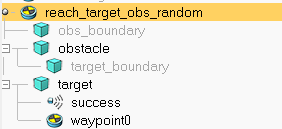
\includegraphics[scale=0.5]{assets/early-work/obs-random-scene-hierarchy.png}
    \caption{`ReachObs\_Random' Scene Hierarchy}
  \end{subfigure}
  \hfill
  \begin{subfigure}{0.45\linewidth}
    \centering
    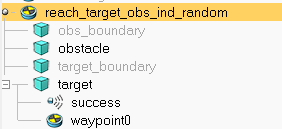
\includegraphics[scale=0.5]{assets/early-work/obs-ind-random-scene-hierarchy.png}
    \caption{`ReachObs\_IndRandom' Scene Hierarchy}
  \end{subfigure}
  \caption{Reaching Task with an Obstacle}\label{fig:reach-obs-random}
\end{figure}\todo[color=blue]{smaller?} 

\subsection{Running the Task}
There were a few interesting things of note happening on this task. 

I used the unchanged reaching policy from earlier\todo{ref}. Unsurprisingly this did not perform amazingly, however, there are some important lessons to learn form what we are seeing here. Firstly, I adopted to observe the `minimum distance' to target this time \ref{fig:ro-random-cams}, however the `final distance ' graph can be found in the appendix \todo[color=green]{link appendix}. 

\subsubsection{Why is `IndRandom' just worse?}\todo{not sure actually}
I did not include any figures here as there were too many\todo{should i include figures here}, however some nice ones can be found in \todo{ref the appendix}. To summarise: the models on this version of the task seems to have its `distance' graphs translated slightly up (around $0.1$ metres) while the success rate is halved compared to `Random'. 

This is unlikely due to the difference in task creation, which explained in \ref{subsec:ro-creating-the-task}. This is because even if their generation strategies are different the rendered scene will have extremely similar properties and an unchanged model being trained on respective demos from each task shouldn't show a consistent trend like this. 
After making sure the demos were correct and the rendered items in the two scenes were indeed identical, I believe this difference is just random variance. While data collection, during a full pass for the task I create $10$ test demos. These demos are then used to load and reload the same exact scenario to test various configurations of trained policies (for example all different epochs, minibatch sizes \ldots). So, by random chance, during the 3 full repeats in this data collection, the tests created for the `IndRandom' task must have been 
slightly more challenging. Creating this slight difference in results, however, the trends are similar so the other conclusions track.

If I have enough time, it might be interesting to evaluate the policies trained from either task with test data generated from demos of both tasks.\todo[color=pink]{the scenes are almost identical do one more run comparing the a policy trained on either task to two sets of test demos??, replace this section with the actual data if done}

\begin{figure}[htpb] % htpb allows all placement
  \centering
  \begin{subfigure}{0.45\linewidth}
    \centering
    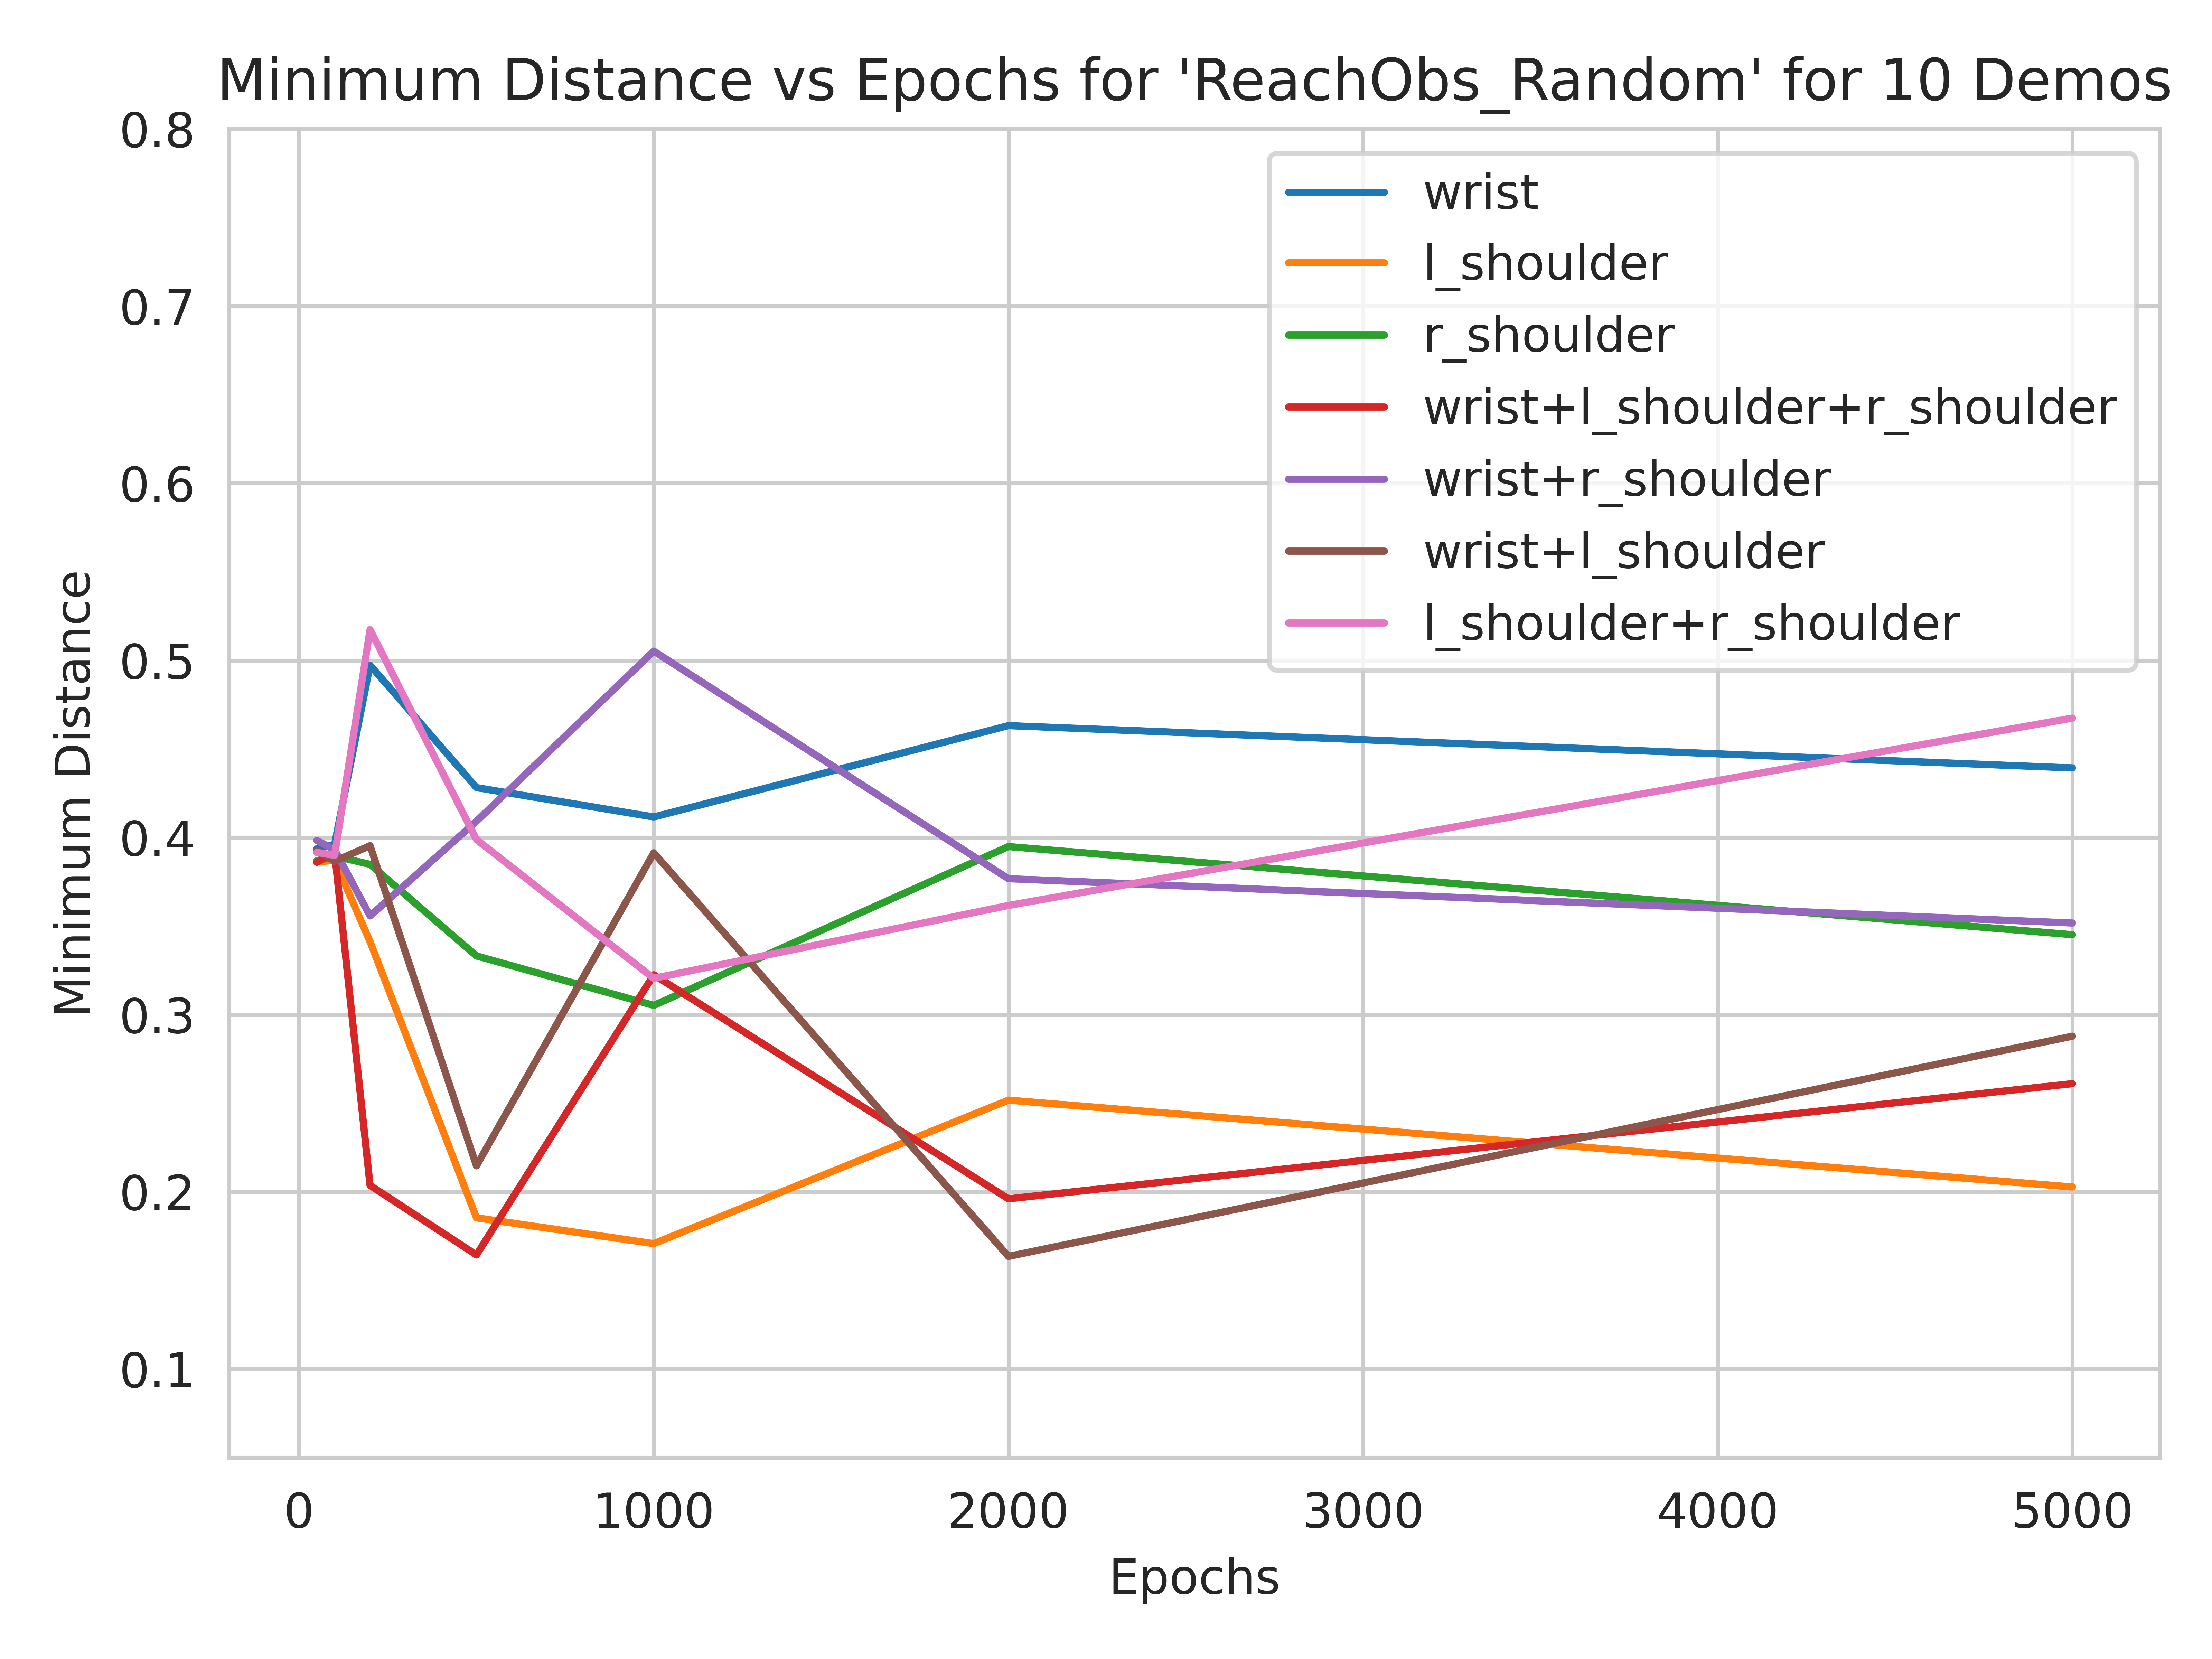
\includegraphics[width=\linewidth]{assets/cam-comb/reach-obs/ro_random-demo-mindist-10demos.png}
    \caption{Minimum Distance to Target}\label{subfig:ro-random-demo-dist-10}
  \end{subfigure}
  \begin{subfigure}{0.45\linewidth}
    \centering
    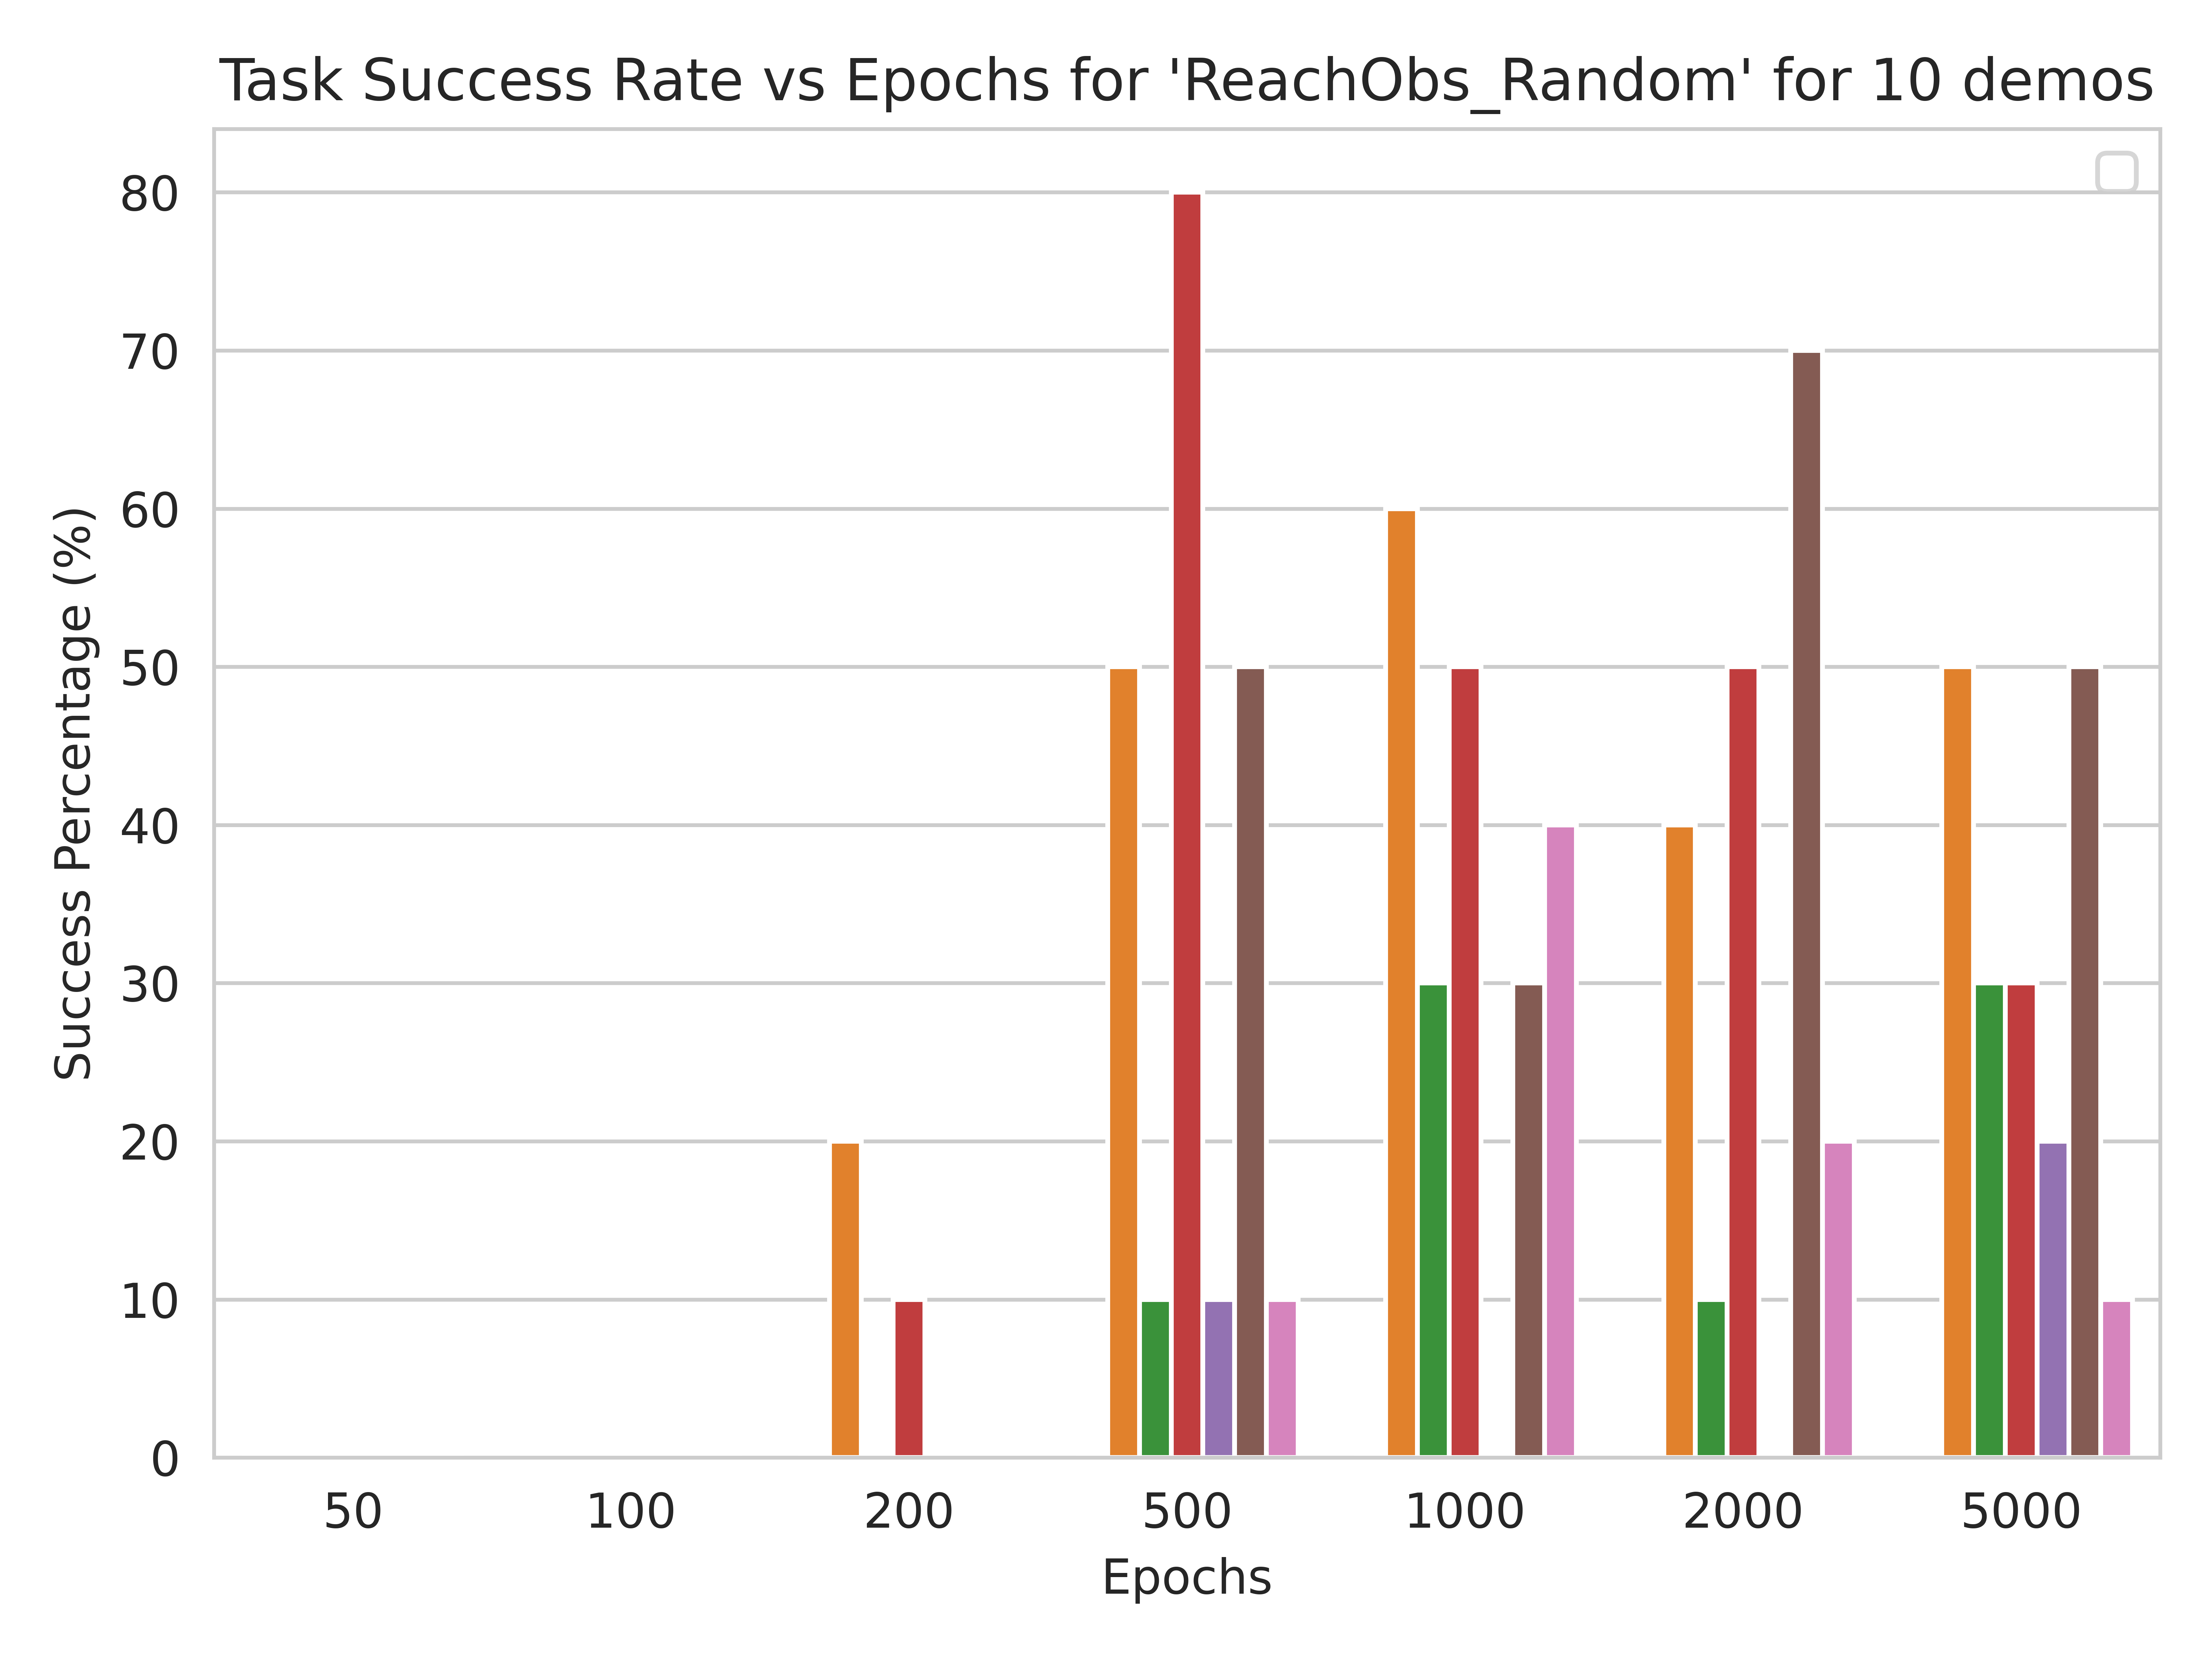
\includegraphics[width=\linewidth]{assets/cam-comb/reach-obs/ro_random-demo-success-10demos.png}
    \caption{Success Rate (\%) of Task}\label{subfig:ro-random-demo-success-10}
  \end{subfigure}
  \caption{Policy trained on 10 demos, using the \emph{demo dataset} from \ref{subsec:grasp-data-loading-changes}}\label{fig:ro-random-demo-cams}
\end{figure}

\subsubsection{Dataset Differences}
I initially was planning on running the system with just the \emph{demo dataset}, however, one of the runs I accidentally included both. After reviewing the data, I realised the \emph{obs dataset} which prematurely flattens and forgets demo boundaries within the data seems to be performing better in this task; see \ref{subfig:ro-random-demo-success-10} and \ref{subfig:ro-random-obs-success-10}. Curiously though, the minimum distance to the target seems to be quite consistent, while the higher success, or course generally leads to a slightly smaller minimum distance.
My theory of why this happens is quite nuanced.\todo[color=purple]{} The \emph{obs dataset} here was trained using \verb|minibatch_size = 32|, the maximum episode length in these demos is $82$. This means that each epoch where the weights of the system are updated, we were exposing it to around one third of the data for a full episode. 
The average episode for this task starts linearly getting near to the side of the obstacle, far away enough to not collide with it, then calculates a non-linear trajectory to curve inwards towards the target for the final bits of the movement.\todo[color=purple]{get a nice video of this for the presentation}. The non-linear part of the demo takes more steps than the linear part. Evident from the fully linear tasks like the grasp and the no obstacle reaching being around $40$ to $60$ steps. This means that the first $30$ ish steps are what the robot takes to move near the obstacle. Therefore, my running theory is that this system was performing better because the task was unintentionally compartmentalised into two sections:
\begin{enumerate}
  \item Reaching to a side of the obstacle
  \item Reaching towards the obstacle.
\end{enumerate}
So, by unintentionally using this batch size we were updating the weights once to reach to a side of the obstacle then to the target. \todo{reread?}. Finding this interesting, I ran more minibatch sizes to see if this was the case (see \ref{apx:Z-ro_random-obs-trials-success}), although, this doesn't seem to be too important once the number of epochs increase, at lower epochs the success rate decreases across the board for larger batch sizes. Although, this is not conclusive, and it might not be ideal nitpicking every demo to specifically train each network, I thought this was an interesting property of sequential batching, even if there is no mechanism to explicitly take care of sequencing in the policy.

\begin{figure}[htpb] % htpb allows all placement
  \centering
  \begin{subfigure}{0.45\linewidth}
    \centering
    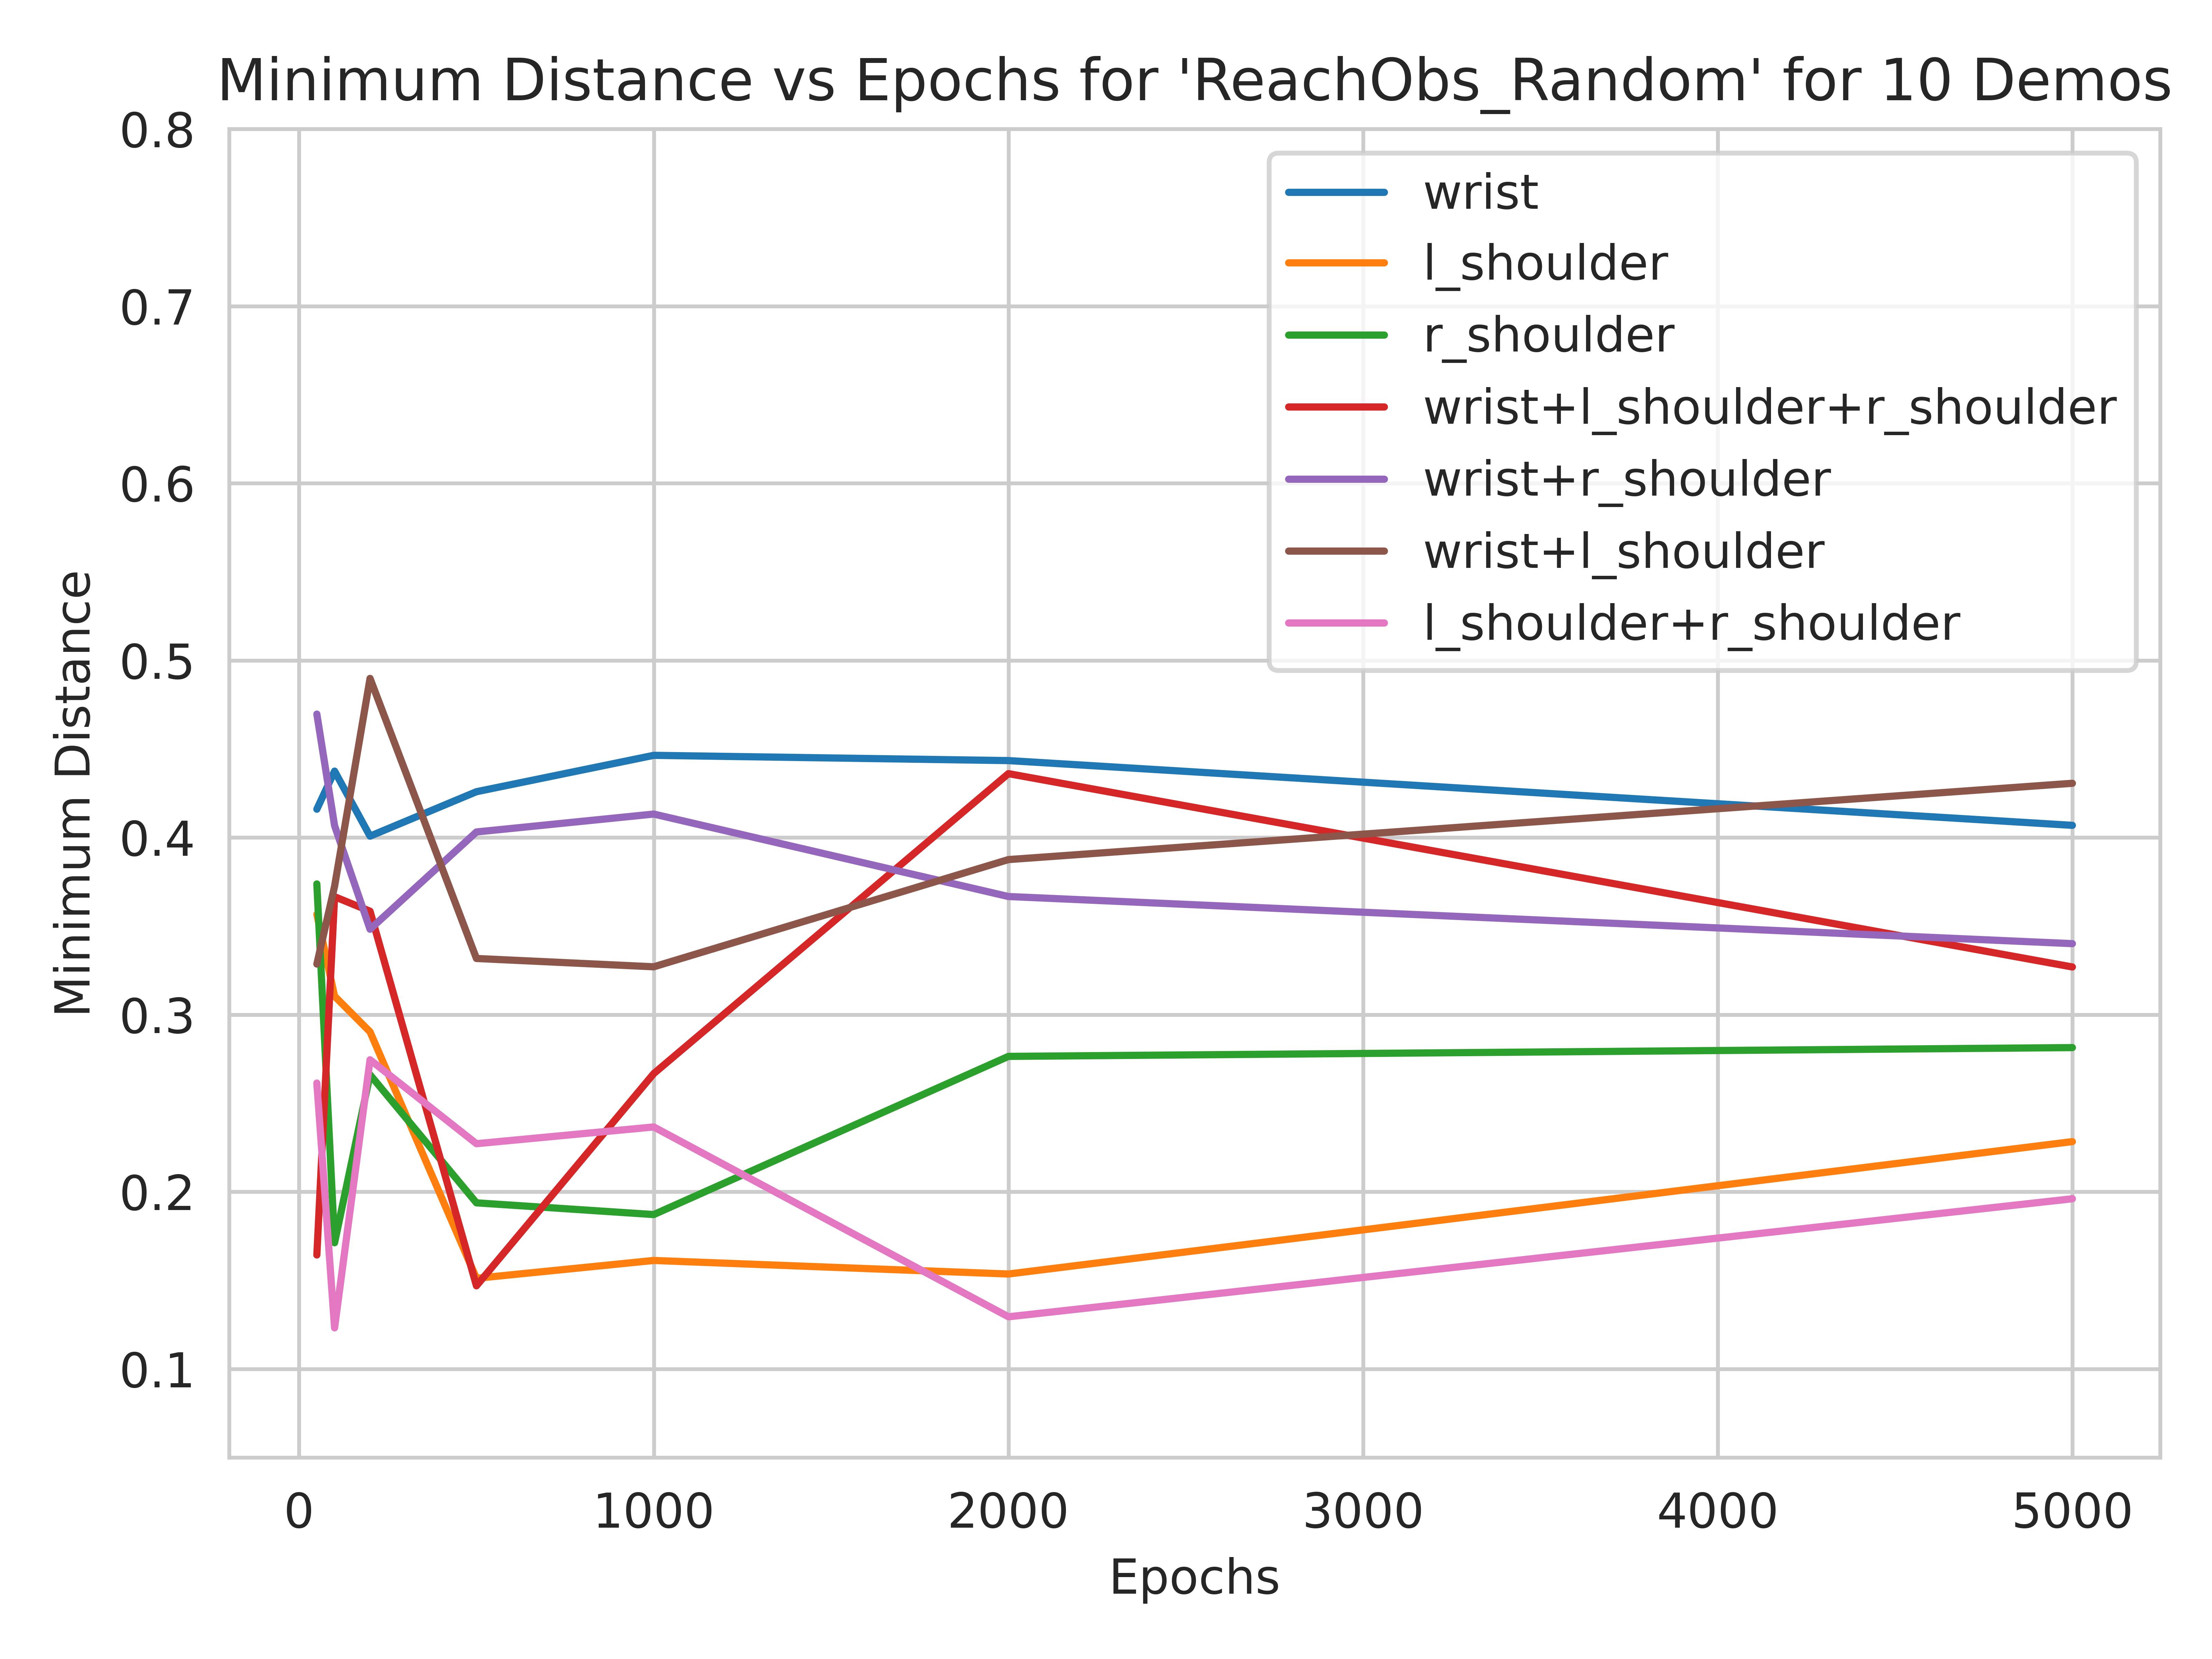
\includegraphics[width=\linewidth]{assets/cam-comb/reach-obs/ro_random-obs-mindist-10demos.png}
    \caption{Minimum Distance to Target}\label{subfig:ro-random-obs-dist-10}
  \end{subfigure}
  \begin{subfigure}{0.45\linewidth}
    \centering
    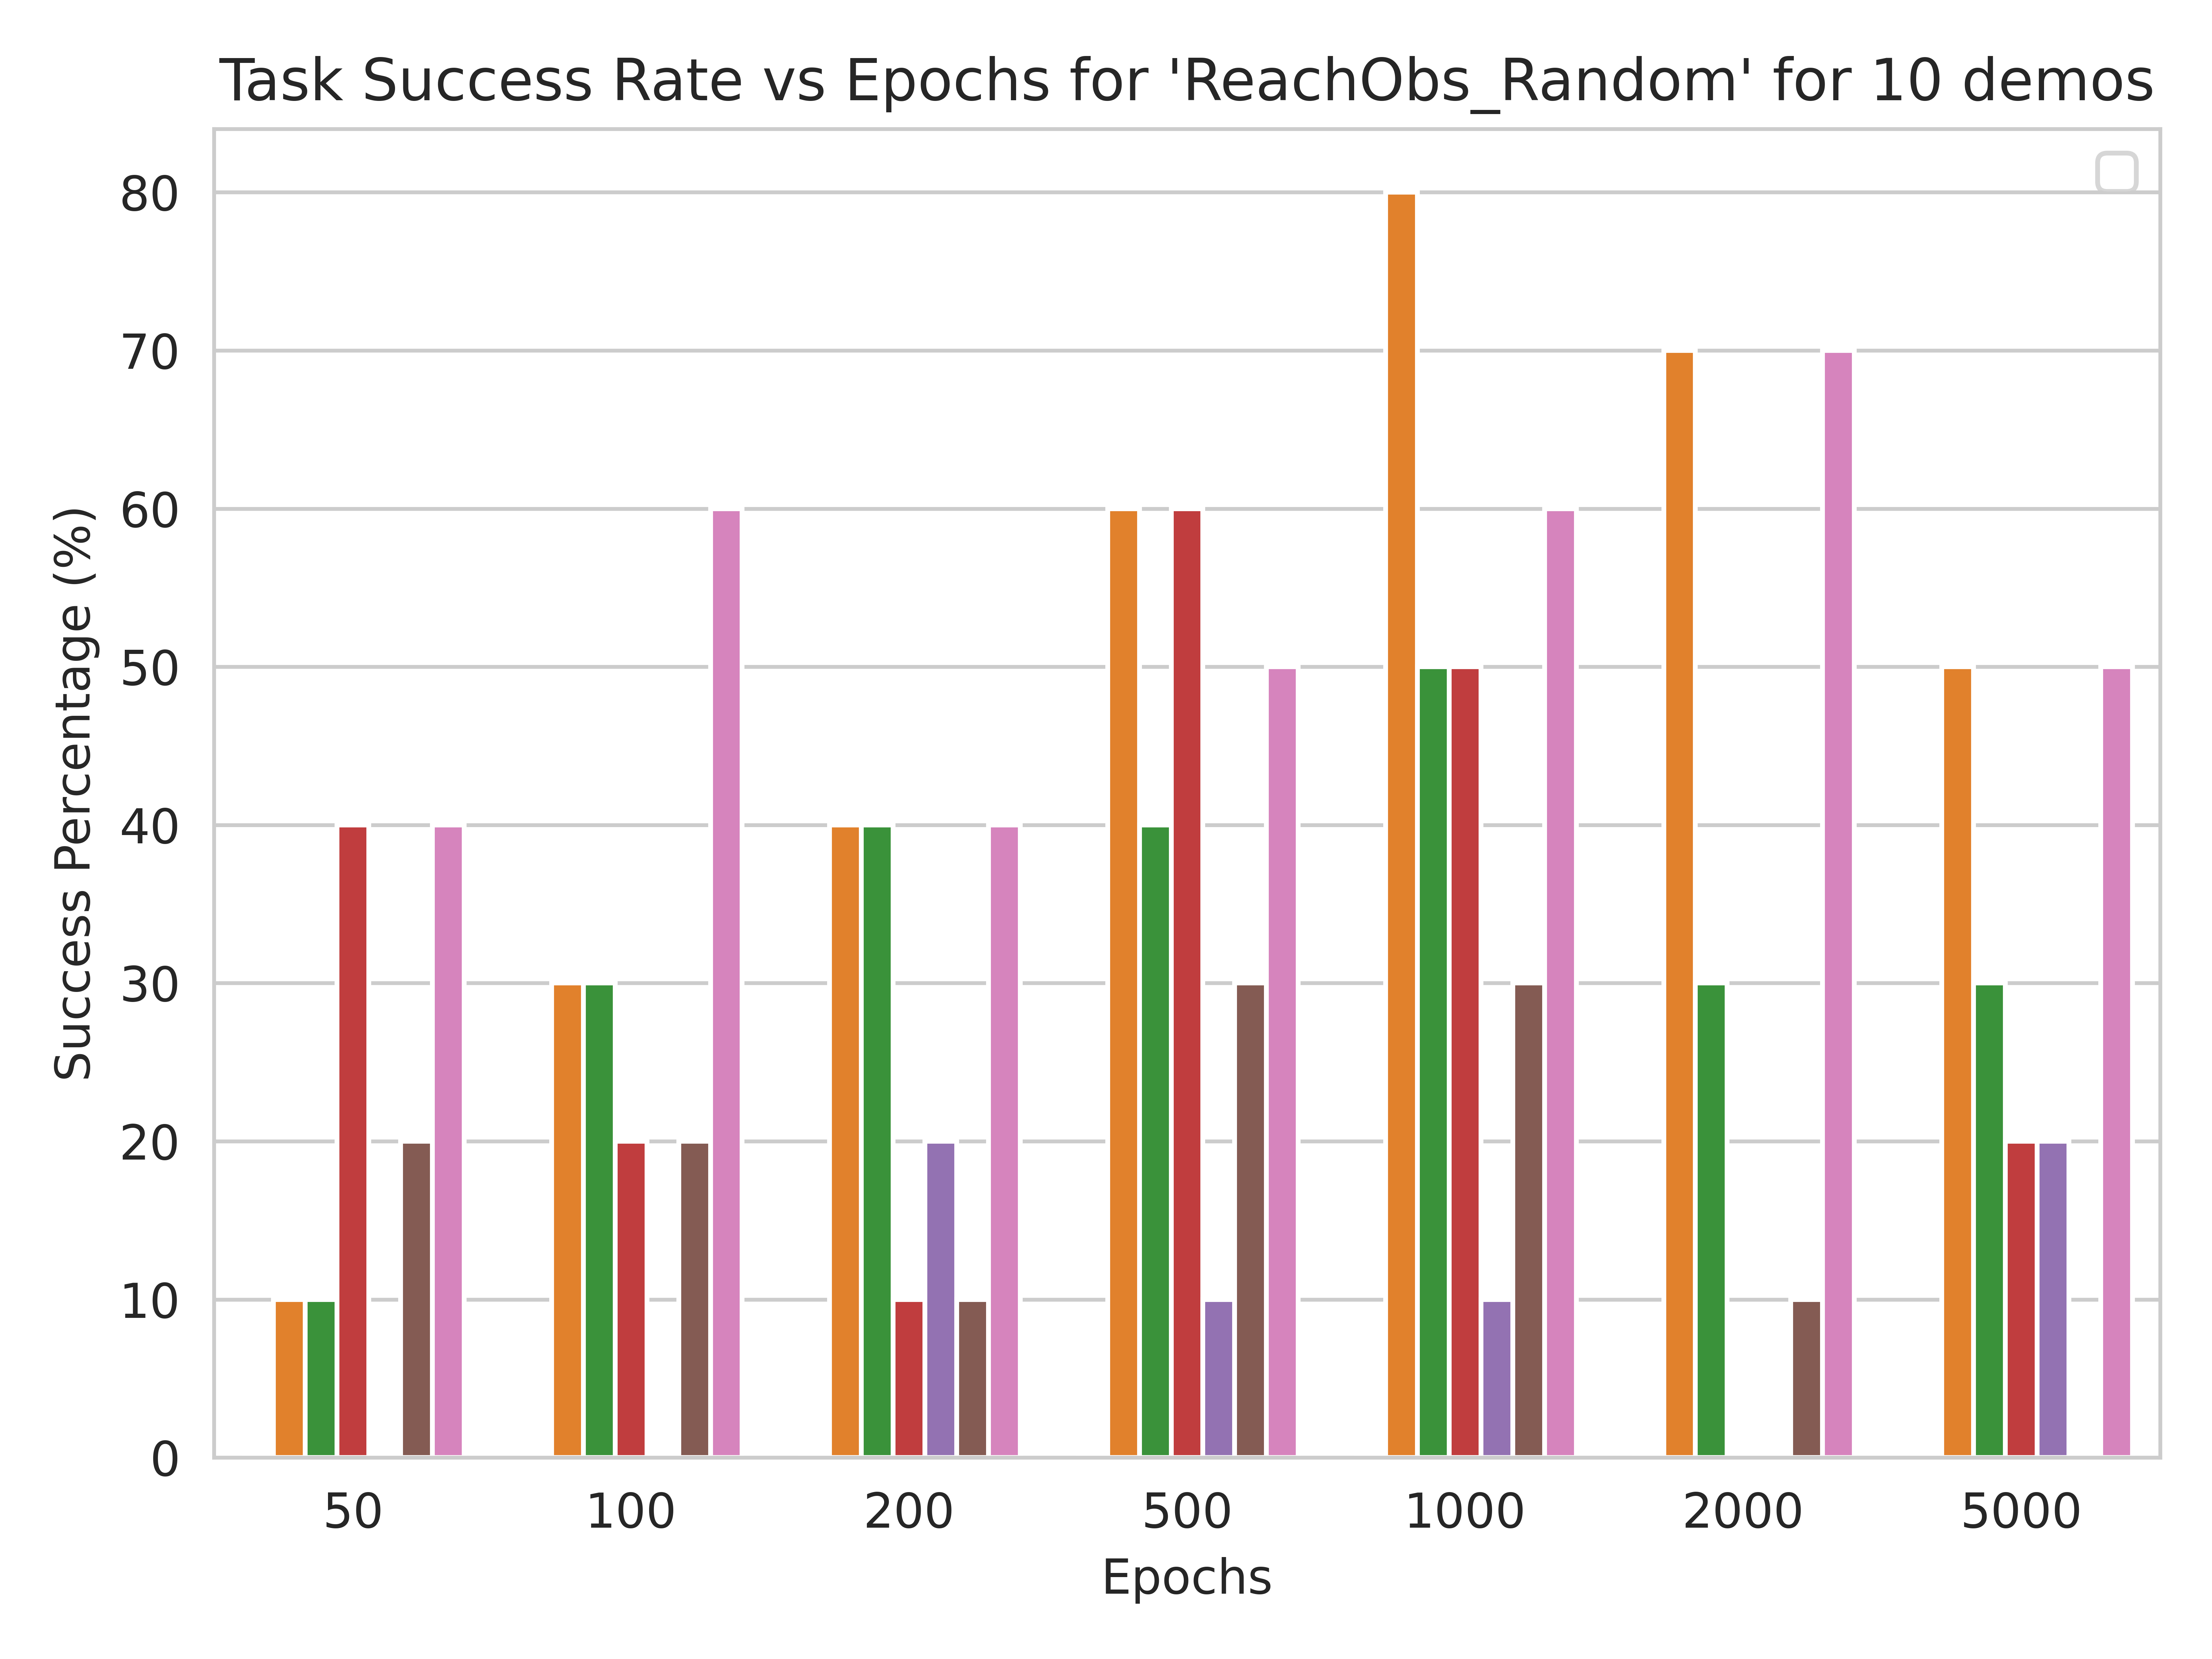
\includegraphics[width=\linewidth]{assets/cam-comb/reach-obs/ro_random-obs-success-10demos.png}
    \caption{Success Rate (\%) of Task}\label{subfig:ro-random-obs-success-10}
  \end{subfigure}
  \caption{Policy trained on 10 demos, using the \emph{obs dataset} from \ref{subsec:reach-data-loading}}\label{fig:ro-random-obs-cams}
\end{figure}

\subsubsection{Wrist Camera Alone isn't Enough}
Although, success rate graph looks nice at first glance, there is a distinct lack of blue; which is the wrist camera. Looking at the minimum distance the wrist achieves (around slightly less than$0.45$) we can see what it does a very good job of going around to the side of the obstacle (as the target is around $0.5$ metres from the obstacle), however, would struggle to make the last steps in touching the target. This is mostly due to the fact that the demonstrations (which are provided by RLBench) are not necessarily pointing the wrist of the robot towards the target. This means all the wrist camera sees once it is past the obstacle is the table (a static view) which means it will likely be out of distribution and do some random movement. It was generally the case that the demo provided would take a wide swing around the obstacle, and almost every wrist rollout I managed to witness, it would just keep slinging the arm away -which is why the final distance graphs were very skewed; even more so for the wrist camera policies.

The other policies that included the wrist features were also prone to these, however sometimes the assisting camera (left or right shoulder would pick something up) and course-correct.

\subsubsection{`Looking' in Demonstrations}\todo{haven't done this yet}\label{ew-looking-at-target}
Another solution might be to experiment with the demonstration system to make sure we are pointing the wrist camera (so, the gripper of our robot) towards its target as a demonstration trajectory is calculated. Playing around this idea, I tried changing the demo calculations. However, issues with precalculation of trajectories and basing that off the grippers pose proved challenging to add this information naturally to demonstration that are given.

If we can't implicitly encode the `looking' information through the demonstration that means we will have to inject this information into our agent some other way and teach it to \emph{actively look} for the target. Following previous works such as \todo{find some prior info tracking works add ref} where object priors are incorporated into the learning or with attention mechanisms that figure out what is important in a task without prior object information \todo[color=red]{not quite sure what i meant by attention here, remove?}.  

\subsubsection{Other Cameras}\todo{rename}
So, we can confirm that the wrist camera alone is not sufficient \todo{ref}, and the combination of wrist and other cameras are almost always better as more coverage of the workspace guarantees less occlusions and more information the agent can work with to make decisions. It was clear that the wrist camera alone wasn't going to cut it unless it learnt to look towards the target. Combining these ideas I moved onto the next section.

\subsection{Attending on a Camera in Given Combination}
First idea bordering on `active vision' was to selectively accept the encoding from a single camera depending on what it was seeing. So, not necessarily looking around, but accepting the inputs from one of the cameras it has access to, guided by some prior information.

\subsubsection{The Colour Score}

\subsection{Score Weighted Features}
Given a set of RGB views, at least two is needed for this policy to act differently than tha others, the idea was to score them and weight them according to their perceived \emph{utility}, the easiest metric was the colour. For every view, $\mathcal{V}$; in our batch, $B$, we calculate a scalar \emph{score} where \(\mathcal{V}_{i, x} \in \mathbb{R}^{B \times {v}}, ~{v} \in \{ {RGB}_{wrist}, ~{RGB}_{left\_shoulder}, ~{RGB}_{right\_shoulder} \}\) the scores are then normalised using softmax: \( \tilde{\mathcal{V}}_{i, x} = \frac{\mathcal{V}_{i, x}}{\sum_{}^{k \in v} \mathcal{V}_{i, k} + 10^{-6}} \) to be a weighing; scalar term $10^{-6}$ being a\todo{a what, what is the correct term?} , indicating which view is the most important at the moment. 




\todo{talk about the implementation of the }
\subsubsection{MultiCNN}
\todo{explaint the implementations, maybe connect to }
\subsubsection{SingleCNN}
I initially though to disconnect the convolutional network, thinking the information can be encoded per view and then fused together to assign better meaning to the given pose. However, with the same logic the scene is still the same scene and encoding features together means that the network will learn to \todo{find a nice way to say the network will learn its fusing in the conv layers. maybe make sure it can}